\section{Actualidad}
\label{sec:tics_ACTUALIDAD}

La relación de los videojuegos con la formación surge en los años 90 y ha
llegado hasta la actualidad en plena efervescencia, siendo aplicados en casi
todos los ámbitos de la educación tanto formal como no formal. Los juegos serios
para el entrenamiento de habilidades se pueden considerar una evolución de las
técnicas de entrenamiento basadas en la realidad virtual que se desarrollaron en
los años 90 y que en la actualidad se han transformado, por su potencial
motivacional, de simulaciones puras a
videojuegos\cite{videojuegos:gonzaleztardon}.

\subsection{Casos de éxito}


\subsubsection{Caso 1. Triage Trainer}
	

\emph{Tipo: } Simulación de entrenamiento.

\emph{Destinatarios: } Médicos, enfermeros, paramédicos y otros rescatistas.

\emph{Contenido} Entrenamiento para evaluar a los pacientes en un lugar de
emergencia.

\emph{Desarrollado por: } TruSim.

\begin{figure}[h!] 
	\centering 
	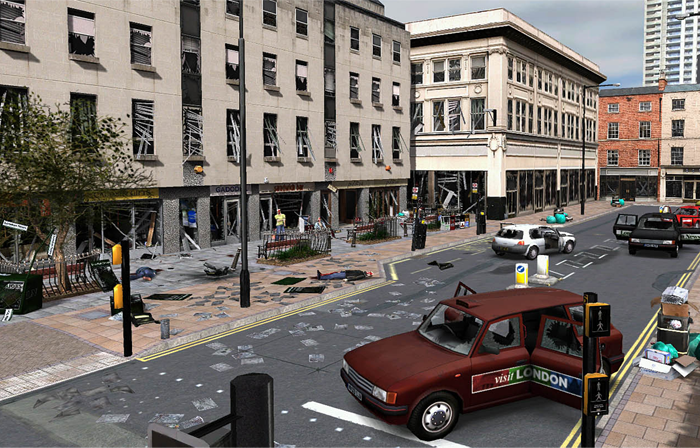
\includegraphics[scale=0.5]{tics/images/triage.png}
	\caption{Ambientación de Triage}
	\label{fig:triage}
\end{figure}

\emph{Visión General: } Triage Trainer se desarrolla en una escena de explosión
en una calle (ver~\ref{fig:triage}) la cual es un incidente mayor, y está
diseñado para formar profesionales que puedan participar en una escena de un
incidente de este tipo (médicos, enfermeros, paramédicos, rescatistas). Los
jugadores deben realizar un triaje, es decir, evaluar el grado de las lesiones
de víctima generadas aleatoriamente utilizando los protocolos y controles
médicos adecuados, además de priorizar a las víctimas para el tratamiento. La
apariencia física de cada víctima es imitada con precisión como los signos
vitales, los síntomas y sobre todo los patrones de tiempo para el deterioro de
las lesiones, es decir, la condición de una víctima cambia de forma realista con
el tiempo (ver~\ref{fig:triage_patient1}.

\begin{figure}[h!]
	\centering 
	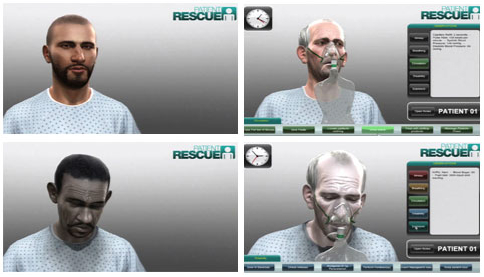
\includegraphics[scale=0.5]{tics/images/patient_side.jpg}
	\caption{Evolución de un paciente en Triage}
	\label{fig:triage_patient1}
\end{figure}

Los jugadores reciben retroalimentación acerca de su rendimiento, incluyendo la
precisión de sus chequeos, si los pacientes fueron priorizados en el orden
correcto y el tiempo que les llevó completar el triaje, en comparación con la de
un experto.

\emph{Evaluación: } La retroalimentación de los participantes que utilizaron
Triage Trainer sugiere que el mismo cumplió exitosamente sus fines. Los
jugadores asociaron su experiencia de juego con su experiencia en el mundo real
y muchos de ellos sentían que realmente estaban allí. Se espera que los
jugadores puedan tomar decisiones bajo presión, lo que ayudará a su desarrollo
cognitivo. También se observó que los jugadores tienden a discutir sus
experiencias con sus compañeros de curso, lo que también podría tener un impacto
en su aprendizaje.

Un elemento que no fue evaluado por TruSim debido a que no era logísticamente
posible fue el impacto de las pruebas en la retención del conocimiento y el
cambio de comportamiento de los jugadores~\cite{education:games}. 


\subsubsection{Caso 2 SimVenture}

\emph{Tipo: } Juego de simulación de negocios.

\emph{Destinatarios: } Personas de 14 a 30 años.

\emph{Contenido: } Las realidades de la creación y funcionamiento de un negocio.

\emph{Desarrollado por: } Venture Simulations.

\emph{Visión General: } En el inicio del
juego(ver~\ref{fig:simventure_tutorial}), a los jugadores se les brinda
informaciones y antecedentes para que que se ubiquen en escena. Ellos deben
empezar a dirigir su propio negocio en su casa de fabricación y venta de
computadoras, mientras deben mantener un trabajo de tiempo completo
independiente. El juego lleva a los jugadores a la ejecución de un negocio en su
propia casa a la extensión del mismo a más locales, lo que requiere contración
de personal. Los jugadores son capaces de avanzar en el juego a través del
aprendizaje de los elementos importantes del empresariado organizadas en cuatro
categorías: organización, ventas/marketing, finanzas y operaciones. Los
jugadores toman decisiones acerca de las actividades dentro de estas áreas y
observan los resultados de sus acciones. 

\begin{figure}[h!]
	\centering 
	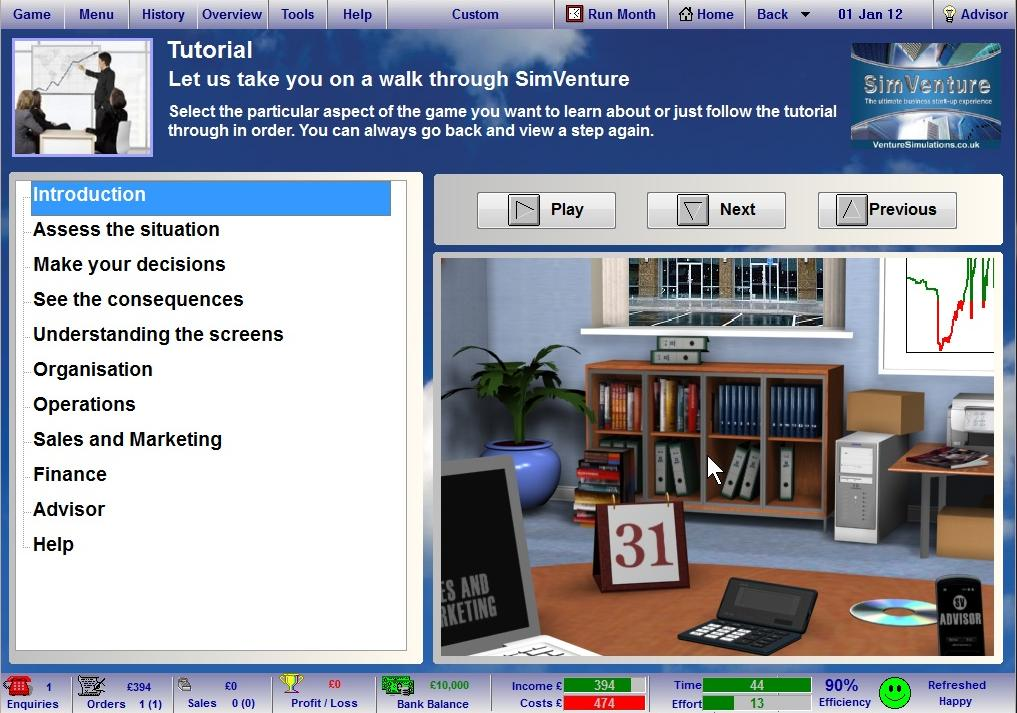
\includegraphics[scale=0.5]{tics/images/simventure-tutorial.jpg}
	\caption{Tutorial de SimVenture}
	\label{fig:simventure_tutorial}
\end{figure}

Los jugadores obtienen retroalimentación sobre un número de diferentes
parámetros. En un nivel básico, se puede simplemente revisar la cantidad de
ingresos que están generando. Además de esto, el éxito puede ser medido por la
cantidad de pedidos que han recibido para sus productos. También se proporciona
retroalimentación visual para representar la eficiencia de la organización y su
felicidad como individuo.

\emph{Evaluación: } Phil Warren, director de estudios de negocios en Snaith
School, ha utilizado SimVenture como complemento al plan de estudios. Según el
mismo, el plan de estudios por lo general sólo requiere que los estudiantes
aprender sobre los diversos elementos diferentes del negocio de forma aislada y
sin embargo, cualquier decisión que se tome en una de las partes de un negocio
tiene efecto en las demás. SimVenture se vió como una oportunidad de aplicar los
conocimientos aprendidos en clase en una actividad práctica, además se observó
que permitir que los estudiantes jueguen en pares da un espacio para la
discusión en torno a las decisiones y aprenden de sus errores
juntos~\cite{education:games}.
